\begin{figure}[!htbp]
\centering
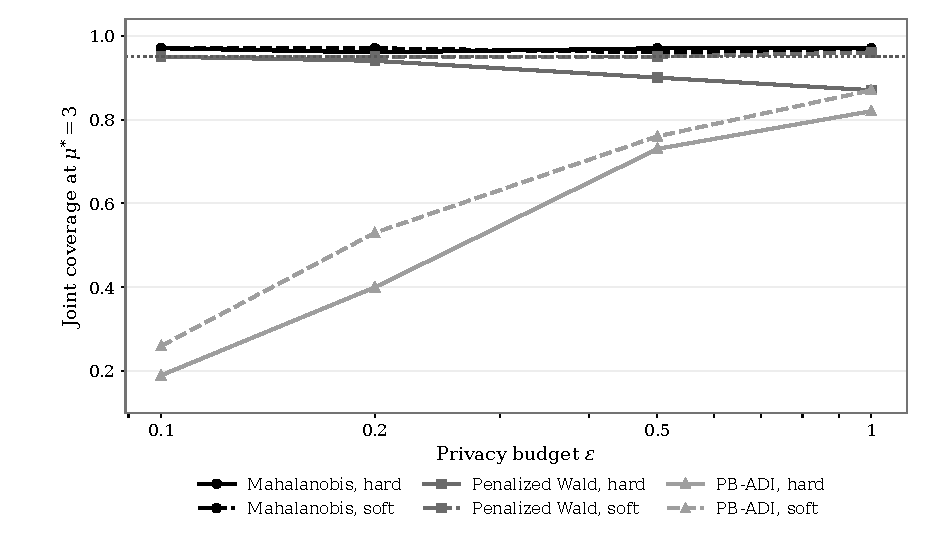
\includegraphics[width=0.78\linewidth]{results/figures/fig_boundary_soft.pdf}
\caption{Joint coverage at $\mu^\ast=3$ under hard (solid) and soft (dashed) clamping. Because the smooth map sends the data into $(L,U)$ the replace-one sensitivities are unchanged, so the two regimes carry exactly the same privacy cost and the only difference between them is the differentiability of the clamp; the clamp type is applied to the release, the acceptance region, the point estimator and the resampler alike. The dotted line is the finite-$R$ bound $0.95025$. Each cell uses $100$ replications, so the Monte Carlo standard error near $0.95$ is $0.022$.}
\label{fig:boundary-soft}
\end{figure}
